\section{VALIDATION AND VERIFICATION}\label{sec:valid}
The model was validated through its response to certain simulation conditions. In this section, all simulations are executed for 1500 ticks.

The first simulation was performed using zero initial population and, as the model does not consider births, the number of agents should remain in zero.  The results are presented in \cref{fig:pop0}. Note that the model behaves as expected.

\begin{figure}[H]
        \centering
        \begin{subfigure}[b]{0.3\columnwidth}
            \centering
            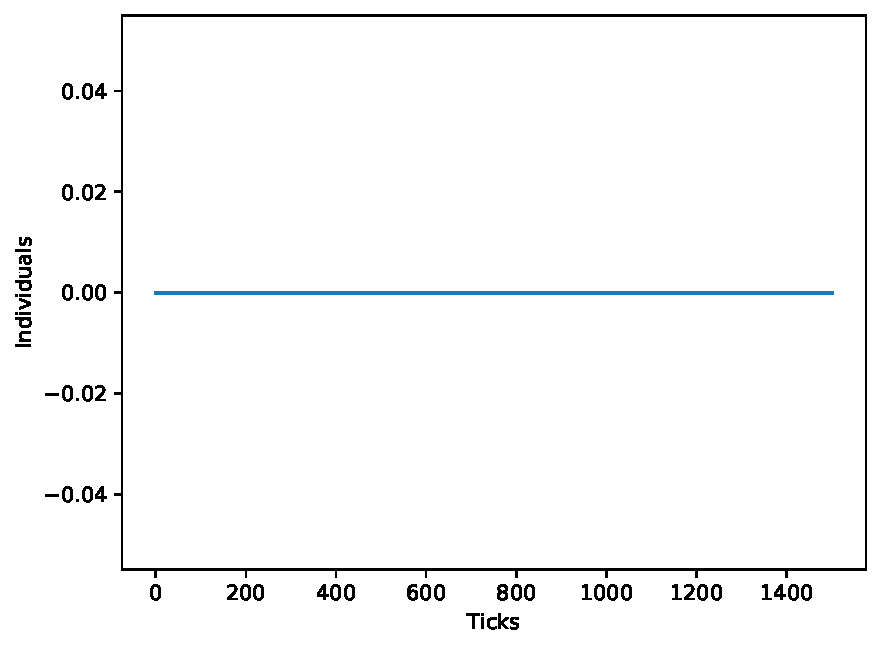
\includegraphics[width=1\columnwidth]{files/population-0-risk.pdf}
            \caption{Risky individuals.}
            \label{subfig:control}
        \end{subfigure} 
        \begin{subfigure}[b]{0.3\columnwidth}
            \centering 
            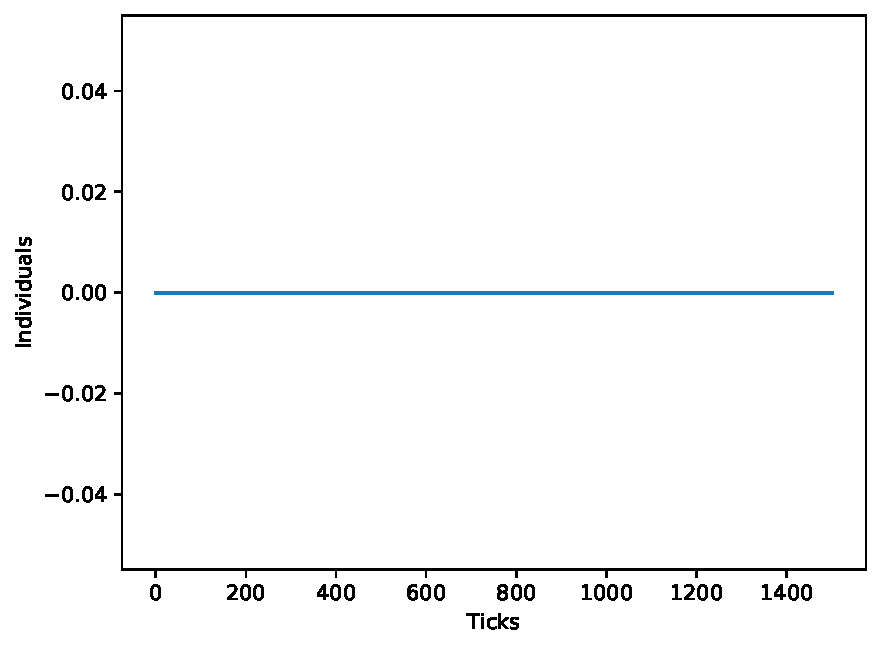
\includegraphics[width=1\columnwidth]{files/population-0-healthy.pdf}
            \caption{Healthy individuals.}
            \label{subfig:sol}
        \end{subfigure}
        \begin{subfigure}[b]{0.3\columnwidth}
            \centering
            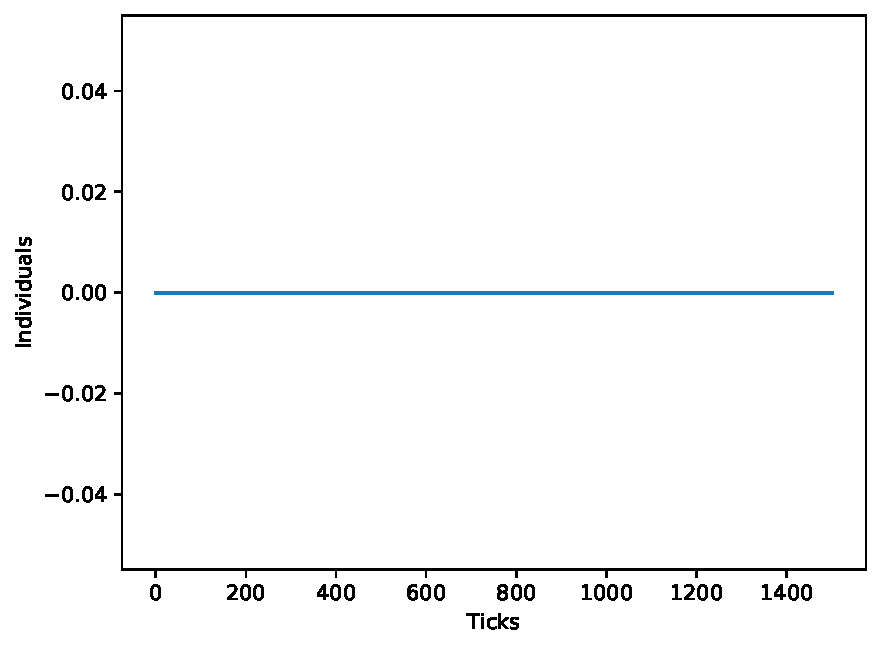
\includegraphics[width=\columnwidth]{files/population-0-diabetes.pdf}
            \caption{Diabetic individuals.}
            \label{subfig:adj}
        \end{subfigure}
        \caption{Results for zero population.}
        \label{fig:pop0}
	\end{figure}

As our model considers that the BMI can only be modified by marital status, if we consider a radius of zero, agents could not marry anyone, since no agent can be found within the radius. Thus, the number of married individuals should remain in zero and the BMI should stabilize rapidly. This can be verified with the obtained results from \cref{fig:rad0}. The used populations were: healthy (71), risky (10) and diabetes (29).
\begin{figure}[H]
        \centering
        \begin{subfigure}[b]{0.3\columnwidth}
            \centering
            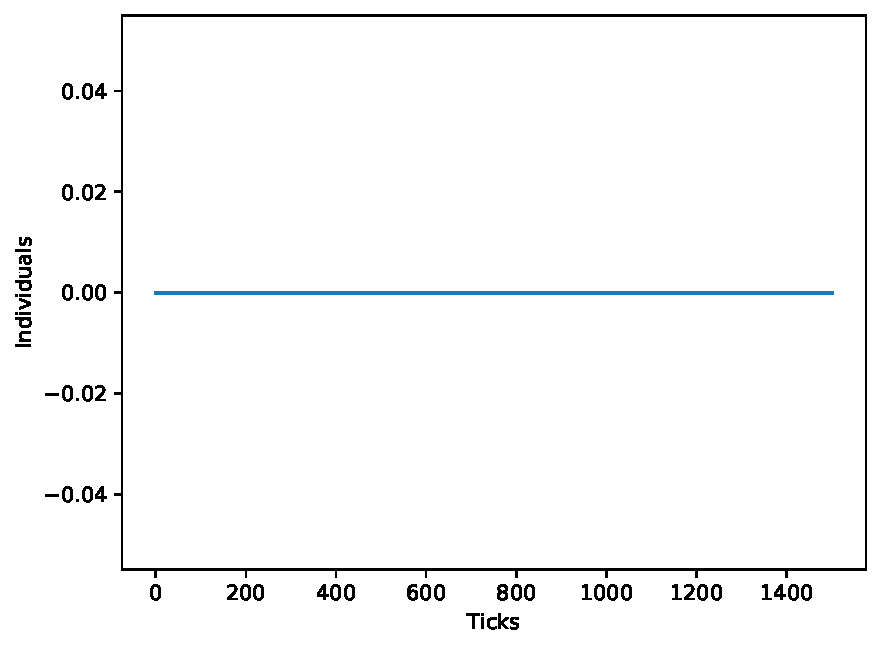
\includegraphics[width=1\columnwidth]{files/radius-0-married.pdf}
            \caption{Number of married agents.}
            \label{subfig:control}
        \end{subfigure} 
        \begin{subfigure}[b]{0.3\columnwidth}
            \centering 
            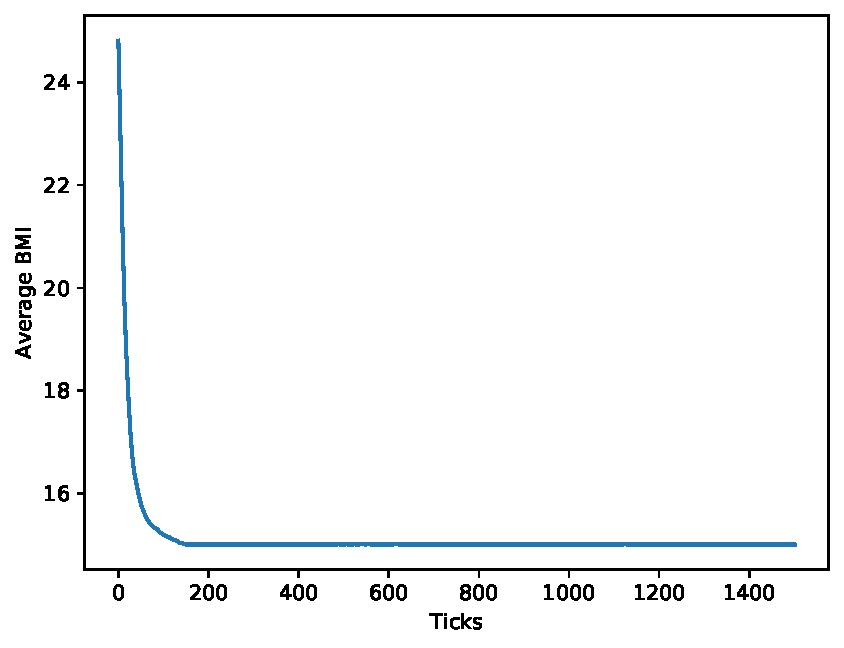
\includegraphics[width=1\columnwidth]{files/radius-0-bmi.pdf}
            \caption{Average BMI.}
            \label{subfig:sol}
        \end{subfigure}
        \caption{Results for zero radius.}
        \label{fig:rad0}
	\end{figure}
	
	Next, we considered a radius of $10^6$. The populations are the same as the previous experiment. \cref{fig:rad1e6} partially supports what was hypothesized, that is, the number of married agents oscillates around the total population size. However, the BMI decreases for unknown reasons.
	\begin{figure}[H]
        \centering
        \begin{subfigure}[b]{0.3\columnwidth}
            \centering
            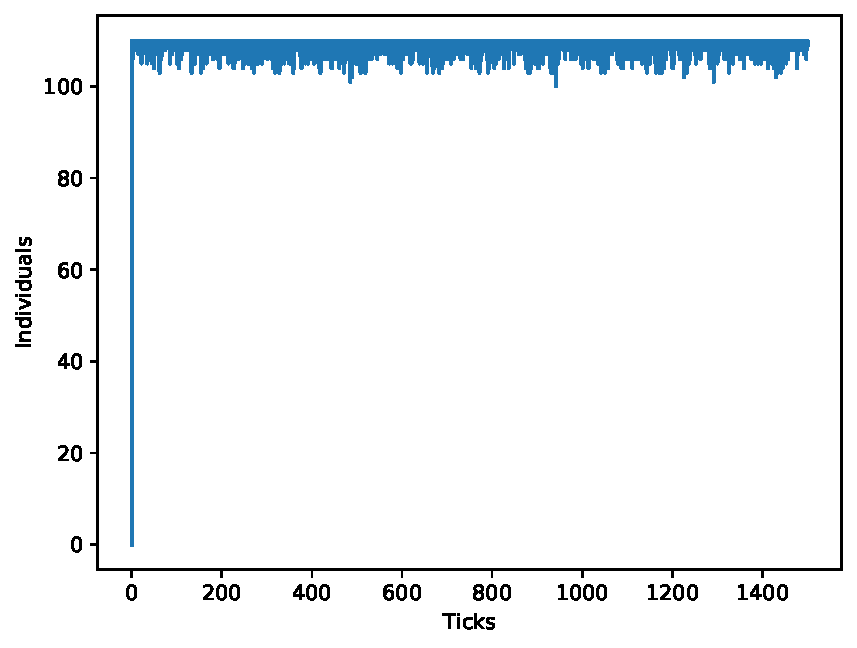
\includegraphics[width=1\columnwidth]{files/radius-1e6-married.pdf}
            \caption{Number of married agents.}
            \label{subfig:control}
        \end{subfigure} 
        \begin{subfigure}[b]{0.3\columnwidth}
            \centering 
            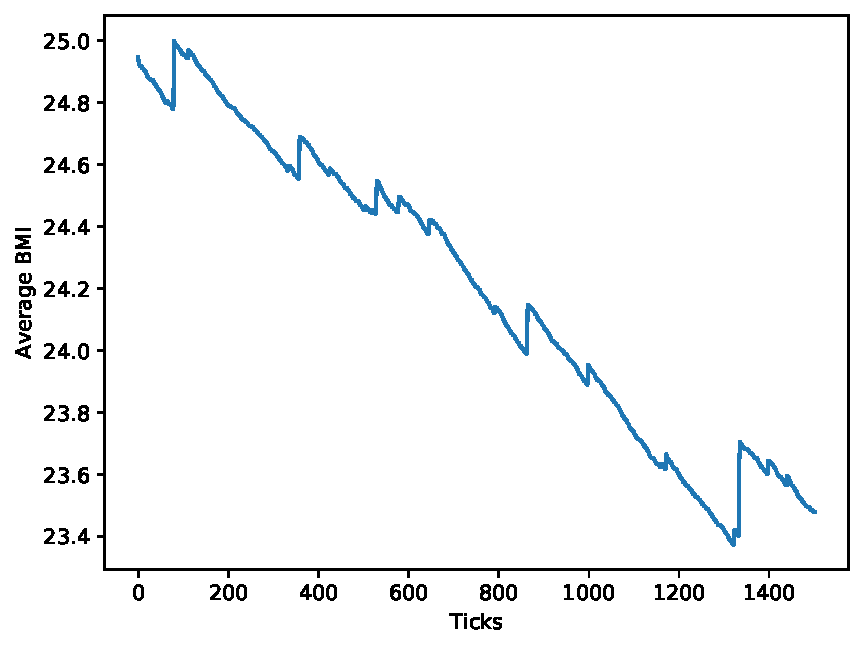
\includegraphics[width=1\columnwidth]{files/radius-1e6-bmi.pdf}
            \caption{Average BMI.}
            \label{subfig:sol}
        \end{subfigure}
        \caption{Results for radius of $10^6$.}
        \label{fig:rad1e6}
	\end{figure}
	
	In \cref{fig:one} the results for the model with only one diabetic individual are presented. Clearly, the agent will change between the diagnoses, contrasting each other.
	\begin{figure}[H]
        \centering
        \begin{subfigure}[b]{0.3\columnwidth}
            \centering
            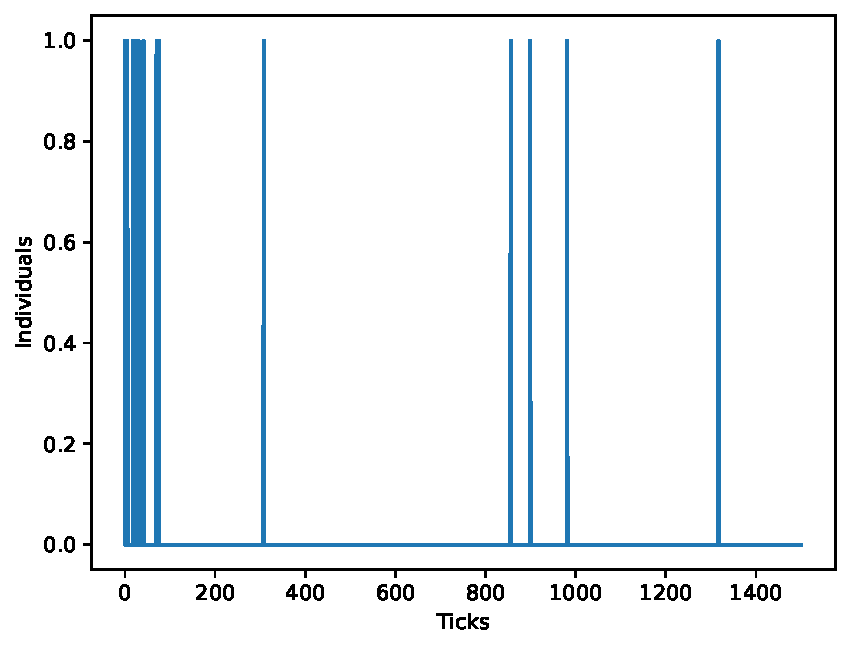
\includegraphics[width=1\columnwidth]{files/diabetes-1-diabetes.pdf}
            \caption{Diabetic.}
            \label{subfig:control}
        \end{subfigure} 
        \begin{subfigure}[b]{0.3\columnwidth}
            \centering 
            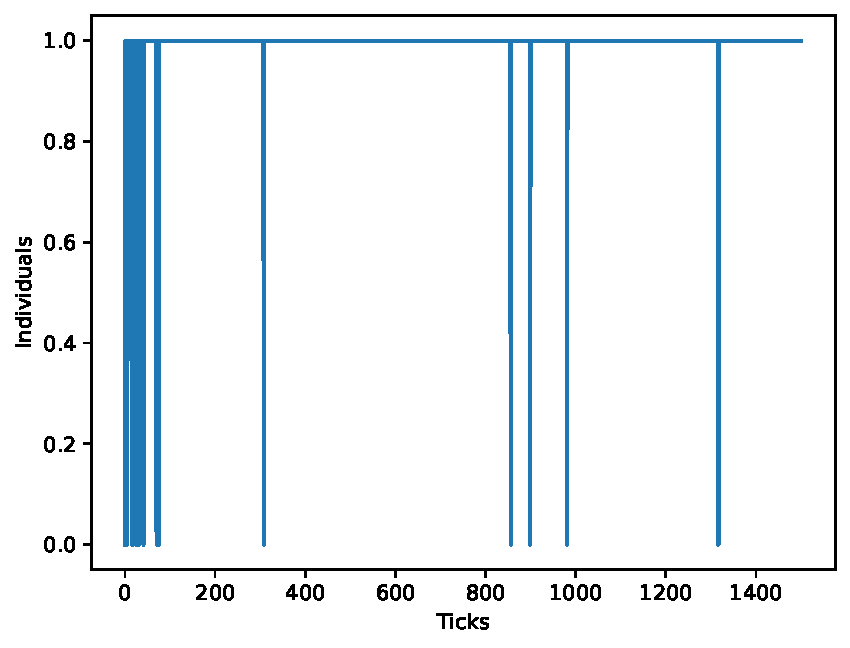
\includegraphics[width=1\columnwidth]{files/diabetes-1-healthy.pdf}
            \caption{Healthy.}
            \label{subfig:sol}
        \end{subfigure}
        \caption{Results for one diabetic individual.}
        \label{fig:one}
	\end{figure}
